%%%%%%%%%%%%%%%%%%%%%%%%%%%%%%%%%%%%%%%%%%%%%%%%%%%%%%%%%%%%%%%%%%%%%%%%%%%%%%%%
\section{Fitting} \label{sec:Fitting}
%%%%%%%%%%%%%%%%%%%%%%%%%%%%%%%%%%%%%%%%%%%%%%%%%%%%%%%%%%%%%%%%%%%%%%%%%%%%%%%%
  \index{Fitting|(}

In addition to the simulation of grazing incidence
X-ray and neutron scattering by
multilayered samples, \BornAgain\ also offers the option to
fit the numerical model to reference data by modifying a selection of
sample parameters from the numerical model.  This aspect
of the software is discussed in the current chapter.

%\cref{sec:FittingGentleIntroducion} gives a short introduction to the
%basic concepts of data fitting. Users familiar with fitting can
%directly proceed to \cref{sec:FittingImplementation}, which details the
%implementation of fittings in
%\BornAgain\ .
\cref{sec:FittingImplementation} details the
implementation of fittings in \BornAgain.
Python fitting examples with detailed
explanations of every fitting step are given in \cref{sec:FittingExamples}. Advanced fitting techniques, including fine tuning of minimization
algorithms, simultaneous fits of different data sets, parameters
correlation, are covered in
\cref{sec:FittingAdvanced}. \cref{sec:FittingRightAnswers} contains some practical advice, which might
help the user to get right answers from \BornAgain\ fitting.


\subsubsection{Implementation in BornAgain} \label{sec:FittingImplementation}

Fitting in  \BornAgain\ deals with estimating the optimum parameters
in the numerical model by minimizing the difference between
numerical and reference data.
%using $\chi^2$  or maximum likelihood methods.
The features include

\begin{itemize}
\item a variety of multidimensional minimization algorithms and strategies.
\item the choice over possible fitting parameters, their properties and correlations.
\item the full control on objective function calculations, including applications of different normalizations and assignments of different masks and weights to different areas of reference data.
\item the possibility to fit simultaneously an arbitrary number of data sets.
\end{itemize}

Figure ~\ref{fig:minimization_workflow} shows the general work flow of a typical fitting procedure.
\begin{figure}[htbp]
\centering
  \resizebox{0.99\textwidth}{!}{%
    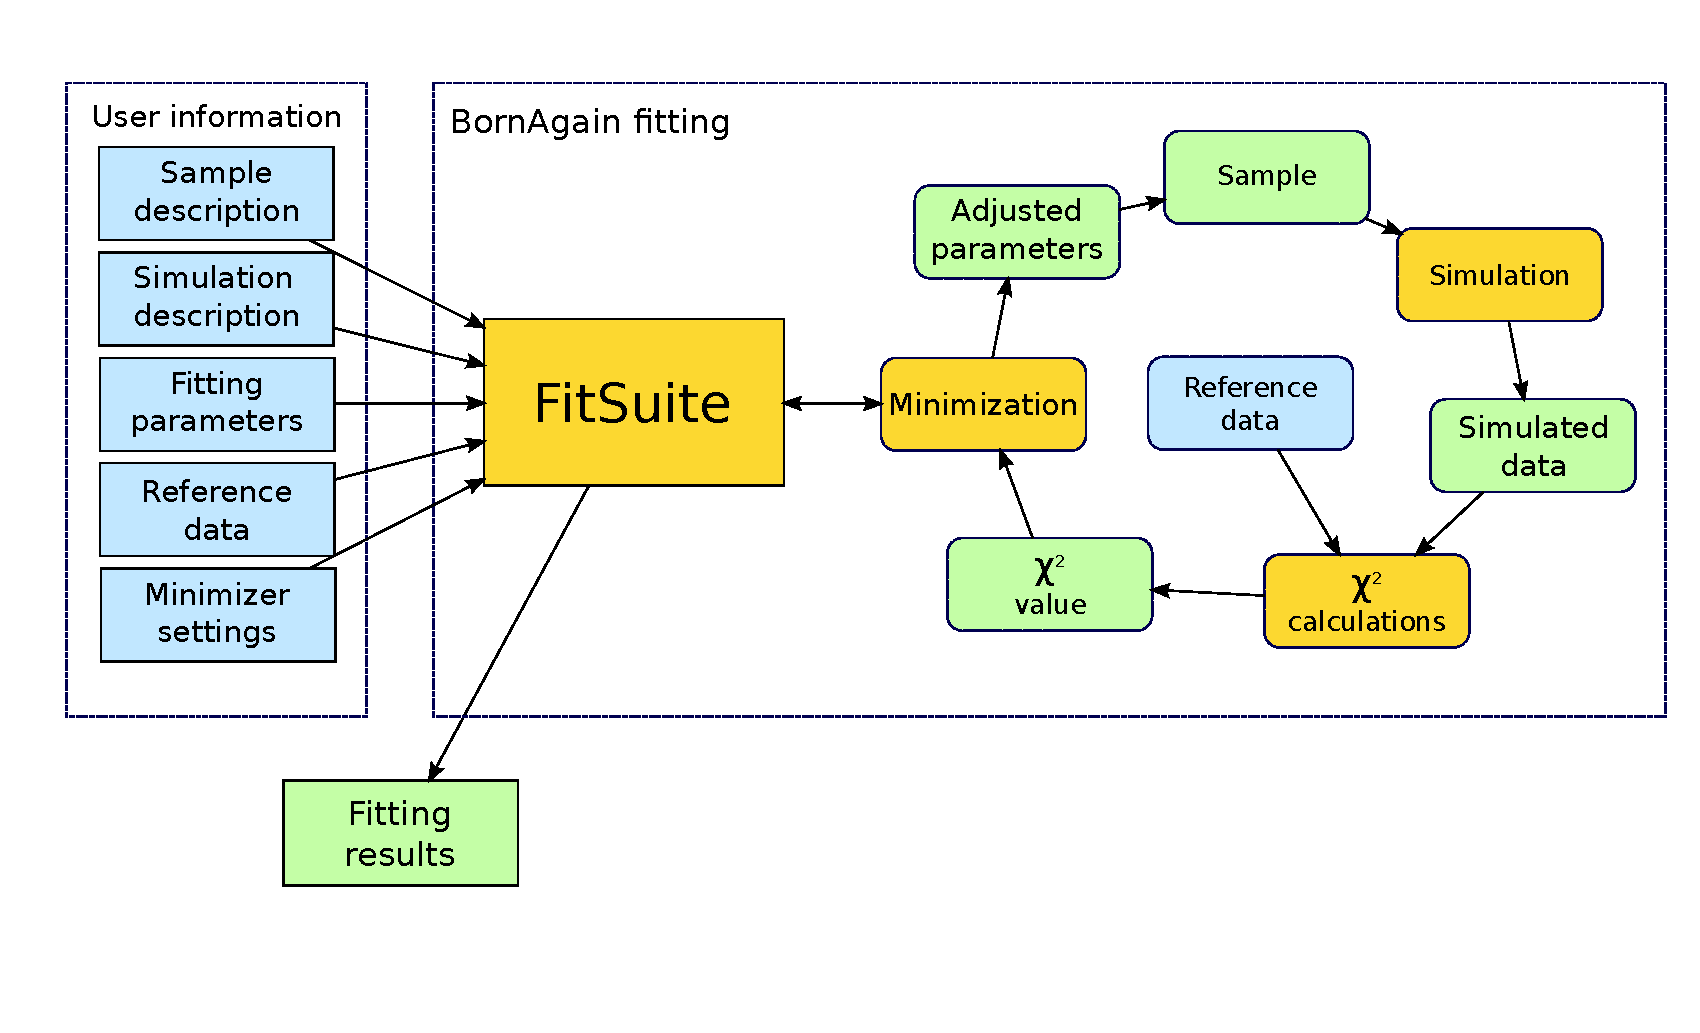
\includegraphics{fig/drawing/minimization_workflow.pdf}}
\caption{
Fitting work flow.
}
\label{fig:minimization_workflow}
\end{figure}

Before running the fitting the user is required to prepare some  data and to
configure the fitting kernel of \BornAgain\ . The required stages are

\begin{itemize}
\item Preparing the sample and the simulation description (multilayer, beam, detector parameters).
\item Choosing the fitting parameters.
\item Loading the reference data.
\item Defining the minimization settings.
\end{itemize}

The class \Code{FitSuite} contains the main functionalities to be used for the fit
and serves as the main interface between the user and the fitting work flow.
The later involves iterations during which

\begin{itemize}
\item The minimizer makes an assumption about the optimal sample parameters.
\item These parameters are propagated to the sample.
\item The simulation is performed for the given state of the sample.
\item The simulated data (intensities) are propagated to the $\chi^2$ module.
\item The later calculates $\chi^2$ using the simulated and reference data.
\item The value of $\chi^2$ is propagated to the minimizer, which makes new assumptions about optimal sample parameters.
\end{itemize}

The iteration process is going on under the control of the selected minimization
algorithm, without any intervention from the
user. It stops
\begin{itemize}
\item when the maximum number of iteration steps has been exceeded,
\item when the function's minimum has been reached within the tolerance window,
\item if the minimizer could not improve the values of the parameters.
\end{itemize}

After the control is returned, fitting results can be retrieved.
They consist in the best $\chi^2$ value found, the corresponding
optimal sample parameters and the intensity map simulated with this set of parameters.

%Details of \Code{FitSuite} class implementation and description of each interface are given in \cref{sec:FitSuiteClass}.
The following parts of this section will detail each of
the main stages necessary to run a fitting procedure.


\subsubsection{Preparing the sample and the simulation description}

This step is similar for any simulation using \BornAgain\ (see \cref{sec:Simulation}). It consists in first characterizing  the geometry of the system: the particles
(shapes, sizes, refractive
indices), the different layers (thickness,
order, refractive index, a possible roughness of the interface), the
interference between the particles and the way they are distributed in
the layers (buried particles or particles sitting on top of a
layer).
Then we specify the parameters of the input beam and of the
output detector.


%===============================================================================
\subsubsection{Choice of parameters to be fitted}
%===============================================================================

In principle, every parameter used in the construction of the sample
can be used as a fitting parameter. For example, the particles'
heights, radii or the layer's roughness or thickness could be selected
using the
parameter pool mechanism.
This mechanism is explained in detail in
\cref{sec:WorkingWithSampleParameters} and it is therefore recommended
to read it before proceeding any further.

The user specifies selected sample parameters as fit parameters using \Code{FitSuite}
and its \Code{addFitParameter} method
\begin{lstlisting}[language=shell, style=commandline]
fit_suite = FitSuite()
fit_suite.addFitParameter(<name>, <initial value>, <step>, <limits>)
\end{lstlisting}
where \Code{<name>} corresponds to the parameter name in the sample's parameter pool.
By using wildcards in the parameter name, a group of sample parameters, corresponding to the given
pattern, can be associated with a single fitting parameter and
fitted simultaneously to get a common optimal value (see \cref{sec:WorkingWithSampleParameters}).

The second parameter \Code <initial value> correspond to the initial value of
the fitting parameter, while the third one
is responsible to the initial iteration steps size.
The last parameter \Code{<AttLimits>} corresponds to
the boundaries imposed on parameter value. It can be
\begin{itemize}
\item \Code{limitless()} by default,
\item \Code{fixed()},
\item \Code{lowerLimited(<min\_value>)},
\item \Code{upperLimited(<max\_value>)},
\item \Code{limited(<min\_value>, <max\_value>)}.
\end{itemize}
where \Code{<min\_value>} and \Code{<max\_value>} are
double values corresponding to the lower and higher boundary, respectively.


%===============================================================================
\subsubsection{Associating reference and simulated data}
%===============================================================================

The minimization procedure deals with a pair of reference data (normally
associated with experimental data) and the theoretical model (presented by the sample and the simulation descriptions).

We assume that the experimental data are a two-dimensional intensity
matrix as function of the output scattering
angles $\alpha_f$ and $\phi_f$ (see \cref{fig:multil3d}).
The user is required to provide the data in the form of an ASCII file
containing an axes
binning description and the intensity data itself.
\vspace*{2mm}

\Note
{We recognize the importance of supporting the most common data formats. We are going to provide
this feature in the following releases and welcome users' requests on this subject.}

To associate the simulation and the reference data to the fitting engine, method \newline
\Code{addSimulationAndRealData} has to be used as shown
\begin{lstlisting}[language=python, style=eclipseboxed,numbers=none]
fit_suite = FitSuite()
fit_suite.addSimulationAndRealData(<simulation>, <reference>, <chi2_module>)
\end{lstlisting}

Here \Code{<simulation>} corresponds to a \BornAgain\ simulation object
with the  sample, beam and detector fully defined, \Code{<reference>}
corresponds to the experimental data object obtained from the ASCII file and \Code{<chi2\_module>} is an optional parameter for advanced
control of $\chi^2$ calculations.

It is possible to call this given method more than once to submit more than one pair of
\Code{<simulation>, <reference>} to the fitting procedure.
In this way, simultaneous fits of
some combined data sets are performed.

By using the third parameter, \Code{<chi2\_module>}, different normalizations and weights
can be applied to give user full control of the way $\chi^2$ is calculated.
This feature will be explained in \cref{sec:FittingAdvanced}.


%===============================================================================
\subsection{Minimizer settings}
%===============================================================================

\BornAgain\ contains a variety of minimization engines from \Code{ROOT} and \Code{GSL}
libraries. They are listed in Table~\ref{table:fit_minimizers}.
By default \Code{Minuit2} minimizer with default settings will be used and no additional
configuration needs to be done.
The remainder of this section explains some of the expert settings, which can be applied to get better
fit results.

The default minimization algorithm can be changed using
\Code{MinimizerFactory} as shown below
\begin{lstlisting}[language=python, style=eclipseboxed,numbers=none]
fit_suite = FitSuite()
minimizer = MinimizerFactory.createMinimizer("<Minimizer name>","<algorithm>")
fit_suite.setMinimizer(minimizer)
\end{lstlisting}

where \Code{<Minimizer name>} and \Code{<algorithm>} can be chosen from the first and
second column of Table~\ref{table:fit_minimizers} respectively.
The list of minimization algorithms implemented in \BornAgain\
can also be obtained using \Code{MinimizerFactory.printCatalogue()} command.


\begin{table}[h]
  \small
\centering
\begin{tabular}{@{}lll@{}}
\hline
\hline
\textbf{Minimizer name} & \textbf{Algorithm} & \textbf{Description}\\
\hline
\Code{Minuit2} \cite{MinuitURL} & \Code{Migrad} & According to
\cite{mntutorial} best minimizer for nearly all functions,\\
 & & variable-metric method with inexact line search, \\
 & & a stable metric updating scheme,\\
 & &  and checks for positive-definiteness.\\
\hline
                                       & \Code{Simplex} & simplex method of
                                       Nelder and Mead\\
 & & usually slower than \Code{Migrad}, \\
 &  & rather robust with respect to gross fluctuations in the\\ & &  function
 value, gives no reliable information about \\ & &  parameter errors, \\
\hline
                                       & \Code{Combined} & minimization with
                                       \Code{Migrad} \\
                                       & & but switches to Simplex if
                                       Migrad fails to converge.\\
\hline
                                       & \Code{Scan} &  not intended to
                                       minimize, just scans the
                                       function,\\
                                       & &  one parameter at a
                                       time, retains the best value
                                       after\\ &  & each scan\\
\hline
                                       & \Code{Fumili} & optimized
                                       method for least square and log
                                       likelihood\\ & &  minimizations \\
\hline
\Code{GSLMultiMin} \cite{GSLMultiMinURL} & \Code{ConjugateFR} & Fletcher-Reeves conjugate gradient
  algorithm,\\
\hline
& \Code{ConjugatePR} & Polak-Ribiere conjugate gradient algorithm,\\
\hline
& \Code{BFGS} & Broyden-Fletcher-Goldfarb-Shanno algorithm,\\
\hline
& \Code{BFGS2} & improved version of BFGS,\\
\hline
& \Code{SteepestDescent} & follows the downhill gradient of the function at each step\\
\hline
\Code{GSLLMA} \cite{GSLMultiFitURL} & & Levenberg-Marquardt
Algorithm\\
\hline
\Code{GSLSimAn} \cite{GSLSimAnURL}& & Simulated Annealing Algorithm\\
\hline
\hline
\end{tabular}
\caption{List of minimizers implemented in \BornAgain. }
\label{table:fit_minimizers}
\index{Minimizers}
\end{table}

There are several options common to every minimization algorithm, which can be changed
before starting the minimization. They are handled by \Code{MinimizerOptions} class:
\begin{lstlisting}[language=python, style=eclipseboxed, numbers = none]
fit_suite.getMinimizer().getOptions().setMaxFunctionCalls(10)
\end{lstlisting}
In the above code snippet, a number of ``maximum function calls'',
namely the maximum number of times the minimizer is allowed to call the simulation, is limited to 10. %The minimizer will take that number into consideration and will try to limit number of iterations by that value.

There are also expert-level options common for all minimizers as well
as a number of options to tune individual minimization algorithms.
They will be explained in \cref{sec:FittingAdvanced}.


%===============================================================================
\subsection{Running the fitting ant retrieving the results}
%===============================================================================

After the initial configuration of \Code{FitSuite} has been performed, the fitting
can be started using the command
\begin{lstlisting}[language=python, style=eclipseboxed, numbers = none]
fit_suite.runFit()
\end{lstlisting}

Depending on the complexity of the sample and the number of free sample parameters the fitting
process can take from tens to thousands of iterations. The results of the fit can
be printed on the screen using the command
\begin{lstlisting}[language=python, style=eclipseboxed, numbers = none]
fit_suite.printResults()
\end{lstlisting}
\cref{sec:FittingExamples} gives more details about how to access the fitting results.


%===============================================================================
\subsection{Basic Python fitting example} \label{sec:FittingExamples}
%===============================================================================

In this section we are going to go through a complete example of
fitting using \BornAgain. Each  step will be associated with a
detailed piece of code written in Python.
The complete listing of
the script is given in Appendix (see Listing~\ref{PythonFittingExampleScript}).
The script can also be found at
\begin{lstlisting}[language=shell, style=commandline]
./Examples/python/fitting/ex002_FitCylindersAndPrisms/FitCylindersAndPrisms.py
\end{lstlisting}

\noindent
This example uses the same sample geometry as in \cref{sec:Example1Python}.
Cylindrical and
prismatic particles in equal proportion are deposited on a substrate layer, with no interference
between the particles. We consider the following parameters to be unkown
\begin{itemize}
\item the radius of cylinders,
\item the height of cylinders,
\item the length of the prisms' triangular basis,
\item the height of prisms.
\end{itemize}

Our reference data are a ``noisy'' two-dimensional intensity
map obtained from the simulation of the same geometry with a fixed
value of $5\,{\rm nm}$ for the height and radius of cylinders and for the
height of prisms which have a 10-nanometer-long side length.
Then we run our fitting using default minimizer settings
starting with a cylinder's height
of $4\,{\rm nm}$, a cylinder's radius of $6\,{\rm nm}$,
a prism's half side of $6\,{\rm nm}$ and a height equal to $4\,{\rm nm}$.
As a result, the fitting procedure is able to find the correct value of $5\,{\rm nm}$
for all four parameters.


%-------------------------------------------------------------------------------
\subsubsection*{Importing Python libraries}
%-------------------------------------------------------------------------------

\begin{lstlisting}[language=python, style=eclipseboxed]
from libBornAgainCore import *
from libBornAgainFit import *
\end{lstlisting}
We start from importing two \BornAgain\ libraries required to create
the sample description
and to run the fitting.

%-------------------------------------------------------------------------------
\subsubsection*{Building the sample}
%-------------------------------------------------------------------------------

\begin{lstlisting}[language=python, style=eclipseboxed, firstnumber=5]
def get_sample(): @\label{script2::get_sample}@
    """
    Build the sample representing cylinders and pyramids on top of substrate without interference.
    """
    # defining materials
    m_air = HomogeneousMaterial("Air", 0.0, 0.0)
    m_substrate = HomogeneousMaterial("Substrate", 6e-6, 2e-8)
    m_particle = HomogeneousMaterial("Particle", 6e-4, 2e-8)

    # collection of particles
    cylinder_ff = FormFactorCylinder(1.0*nanometer, 1.0*nanometer)
    cylinder = Particle(m_particle, cylinder_ff)
    prism_ff = FormFactorPrism3(2.0*nanometer, 1.0*nanometer)
    prism = Particle(m_particle, prism_ff)
    particle_layout = ParticleLayout()
    particle_layout.addParticle(cylinder, 0.5)
    particle_layout.addParticle(prism, 0.5)
    interference = InterferenceFunctionNone()
    particle_layout.setInterferenceFunction(interference)

    # air layer with particles and substrate form multi layer
    air_layer = Layer(m_air)
    air_layer.addLayout(particle_layout)
    substrate_layer = Layer(m_substrate)
    multi_layer = MultiLayer()
    multi_layer.addLayer(air_layer)
    multi_layer.addLayer(substrate_layer)
    return multi_layer
\end{lstlisting}
The function starting at line~\ref{script2::get_sample} creates a multilayered sample
with cylinders and prisms using arbitrary $1\,{\rm nm}$ value for all size's of particles.
The details about the generation of this multilayered sample are given in \cref{sec:Example1Python}.

%-------------------------------------------------------------------------------
\subsubsection*{Creating the simulation}
%-------------------------------------------------------------------------------
\begin{lstlisting}[language=python, style=eclipseboxed, firstnumber=35]
def get_simulation(): @\label{script2::get_simulation}@
    """
    Create GISAXS simulation with beam and detector defined
    """
    simulation = Simulation()
    simulation.setDetectorParameters(100, -1.0*degree, 1.0*degree, 100, 0.0*degree, 2.0*degree)
    simulation.setBeamParameters(1.0*angstrom, 0.2*degree, 0.0*degree)
    return simulation
\end{lstlisting}
The function starting at line~\ref{script2::get_simulation} creates
the simulation object with the definition of the beam and detector parameters.

%-------------------------------------------------------------------------------
\subsubsection*{Preparing the fitting pair}
%-------------------------------------------------------------------------------
\begin{lstlisting}[language=python, style=eclipseboxed, firstnumber=45]
def run_fitting(): @\label{script2::run_fitting}@
    """
    run fitting
    """
    sample = get_sample() @\label{script2::setup_simulation1}@
    simulation = get_simulation()
    simulation.setSample(sample) @\label{script2::setup_simulation2}@

    real_data = IntensityDataIOFactory.readIntensityData('refdata_fitcylinderprisms.int.gz') @\label{script2::real_data}@
\end{lstlisting}
Lines
~\ref{script2::setup_simulation1}-~\ref{script2::setup_simulation2}
generate the
sample and simulation description and assign the sample to the simulation.
Our reference data are contained in the file \Code{'refdata\_fitcylinderprisms.int.gz'}.
 This reference had been generated by adding noise
on the scattered intensity from a numerical sample with a fixed length of 5~nm for the four fitting
parameters (\idest the dimensions of the cylinders and prisms).
Line ~\ref{script2::real_data} creates the real data object by loading
the ASCII data from the input file.

%-------------------------------------------------------------------------------
\subsubsection*{Setting up \rm\bf{FitSuite}}
%-------------------------------------------------------------------------------
\begin{lstlisting}[language=python, style=eclipseboxed, firstnumber=55]
    fit_suite = FitSuite() @\label{script2::fitsuite1}@
    fit_suite.addSimulationAndRealData(simulation, real_data) @\label{script2::fitsuite2}@
    fit_suite.initPrint(10) @\label{script2::fitsuite3}@
\end{lstlisting}
Line ~\ref{script2::fitsuite1} creates a \Code{FitSuite} object which provides
the main interface to the minimization kernel of \BornAgain\ .
Line ~\ref{script2::fitsuite2} submits simulation description and real data pair to the
subsequent fitting. Line ~\ref{script2::fitsuite3} sets up \Code{FitSuite} to print on
the screen the information about fit progress once per 10 iterations.
\begin{lstlisting}[language=python, style=eclipseboxed, firstnumber=60]
    fit_suite.addFitParameter("*FormFactorCylinder/height", 4.*nanometer, 0.01*nanometer, AttLimits.lowerLimited(0.01)) @\label{script2::fitpars1}@
    fit_suite.addFitParameter("*FormFactorCylinder/radius", 6.*nanometer, 0.01*nanometer, AttLimits.lowerLimited(0.01))
    fit_suite.addFitParameter("*FormFactorPrism3/height", 4.*nanometer, 0.01*nanometer, AttLimits.lowerLimited(0.01))
    fit_suite.addFitParameter("*FormFactorPrism3/length", 12.*nanometer, 0.02*nanometer, AttLimits.lowerLimited(0.01)) @\label{script2::fitpars2}@
\end{lstlisting}
Lines ~\ref{script2::fitpars1}--~\ref{script2::fitpars2} enter the
list of fitting parameters. Here we use the cylinders' height and
radius and the prisms' height and side length.
The cylinder's length and prism half side are initially equal to $4\,{\rm nm}$,
whereas the cylinder's radius and the prism half side length are equal to $6\,{\rm nm}$ before the minimization. The
iteration step is equal to $0.01\,{\rm nm}$ and only the lower
boundary is imposed to be equal to $0.01\,{\rm nm}$.

%-------------------------------------------------------------------------------
\subsubsection*{Running the fit and accessing results}
%-------------------------------------------------------------------------------
\begin{lstlisting}[language=python, style=eclipseboxed, firstnumber=66]
    fit_suite.runFit() @\label{script2::fitresults1}@

    print "Fitting completed."
    fit_suite.printResults()@\label{script2::fitresults2}@
    print "chi2:", fit_suite.getMinimizer().getMinValue()
    fitpars = fit_suite.getFitParameters()
    for i in range(0, fitpars.size()):
        print fitpars[i].getName(), fitpars[i].getValue(), fitpars[i].getError() @\label{script2::fitresults3}@
\end{lstlisting}
Line ~\ref{script2::fitresults1} shows the command to start the fitting process.
During the fitting the progress will be displayed on the screen.
Lines ~\ref{script2::fitresults2}--~\ref{script2::fitresults3} shows different ways of
accessing the fit results.


More details about fitting, access to its results and visualization of
the fit progress using matplotlib libraries can be learned from the
following detailed example
\begin{lstlisting}[language=shell, style=commandline]
./Examples/python/fitting/ex002_FitCylindersAndPrisms/FitCylindersAndPrisms_detailed.py
\end{lstlisting}


%===============================================================================
\subsection{Advanced fitting} \label{sec:FittingAdvanced}
%===============================================================================

\subsubsection{Affecting chi-square calculations}
\MissingSection
\subsubsection{Simultaneous fits of several data sets}
\MissingSection
\subsubsection{Using fitting strategies}
\MissingSection
\subsubsection{Masking the real data}
\MissingSection
\subsubsection{Tuning fitting algorithms}
\MissingSection
\subsubsection{Fitting with correlated sample parameters}
\MissingSection


%===============================================================================
\subsection {How to get the right answer from fitting}
  \label{sec:FittingRightAnswers}
%===============================================================================

%As it has already been mentioned in \cref{sec:FittingGentleIntroducion},
One of the main difficulties in fitting the data with the model
is the presence of multiple
local minima in the objective function. Many problems can cause the
fit to fail, for example:
\begin{itemize}
\item an unreliable physical model,
\item an unappropriate choice of objective function
\item multiple local minima,
\item an unphysical behavior of the objective function, unphysical regions
  in the parameters space,
\item an unreliable parameter error calculation in the presence of
  limits on the parameter value,
\item an exponential behavior of the objective function and the
  corresponding numerical inaccuracies, excessive numerical roundoff
  in the calculation of its value and derivatives,
\item large correlations between parameters,
\item very different scales of parameters involved in the calculation,
\item not positive definite error matrix even at minimum.
\end{itemize}


The given list, of course, is not only related to \BornAgain\
fitting. It remains applicable to any fitting program and any kind of theoretical model.
%To address all these difficulties some amount of manual tuning might be necessary.
 Below we give some recommendations which might help the user to achieve reliable fit results.

\subsection*{General recommendations}
\begin{itemize}
\item initially choose  a small number of free fitting parameters,
\item eliminate redundant parameters,
\item provide a good initial guess for the fit parameters,
\item start from the default minimizer settings and perform some fine tuning after some experience has been acquired,
\item repeat the fit using different starting values for the parameters or their limits,
\item repeat the fit, fixing and varying different groups of parameters,
%\item use \Code{Minuit2} minimizer with \Code{Migrad} algorithm
%  (default) to get the most reliable parameter error estimation,
%\item try \Code{GSLMultiFit} minimizer or \Code{Minuit2} minimizer with \Code{Fumili} %algorithm to get fewer iterations.
\end{itemize}

\Work{... to be continued ...}

%\subsection*{Interpretation of errors.}

\index{Fitting|)}
